\documentclass{beamer}
\mode<presentation>
\usepackage{amsmath}
\usepackage{amssymb}
%\usepackage{advdate}
\usepackage{adjustbox}
\usepackage{subcaption}
\usepackage{enumitem}
\usepackage{multicol}
\usepackage{mathtools}
\usepackage{listings}
\usepackage{float}
\usepackage{graphicx}
\usepackage{url}
\def\UrlBreaks{\do\/\do-}
\usetheme{Boadilla}
\usecolortheme{lily}
\setbeamertemplate{footline}
{
  \leavevmode%
  \hbox{%
  \begin{beamercolorbox}[wd=\paperwidth,ht=2.25ex,dp=1ex,right]{author in head/foot}%
    \insertframenumber{} / \inserttotalframenumber\hspace*{2ex} 
  \end{beamercolorbox}}%
  \vskip0pt%
}
\setbeamertemplate{navigation symbols}{}

\providecommand{\nCr}[2]{\,^{#1}C_{#2}} % nCr
\providecommand{\nPr}[2]{\,^{#1}P_{#2}} % nPr
\providecommand{\mbf}{\mathbf}
\providecommand{\pr}[1]{\ensuremath{\Pr\left(#1\right)}}
\providecommand{\qfunc}[1]{\ensuremath{Q\left(#1\right)}}
\providecommand{\sbrak}[1]{\ensuremath{{}\left[#1\right]}}
\providecommand{\lsbrak}[1]{\ensuremath{{}\left[#1\right.}}
\providecommand{\rsbrak}[1]{\ensuremath{{}\left.#1\right]}}
\providecommand{\brak}[1]{\ensuremath{\left(#1\right)}}
\providecommand{\lbrak}[1]{\ensuremath{\left(#1\right.}}
\providecommand{\rbrak}[1]{\ensuremath{\left.#1\right)}}
\providecommand{\cbrak}[1]{\ensuremath{\left\{#1\right\}}}
\providecommand{\lcbrak}[1]{\ensuremath{\left\{#1\right.}}
\providecommand{\rcbrak}[1]{\ensuremath{\left.#1\right\}}}
\theoremstyle{remark}
\newtheorem{rem}{Remark}
\newcommand{\sgn}{\mathop{\mathrm{sgn}}}
\providecommand{\abs}[1]{\left\vert#1\right\vert}
\providecommand{\res}[1]{\Res\displaylimits_{#1}} 
\providecommand{\norm}[1]{\lVert#1\rVert}
\providecommand{\mtx}[1]{\mathbf{#1}}
\providecommand{\mean}[1]{E\left[ #1 \right]}
\providecommand{\fourier}{\overset{\mathcal{F}}{ \rightleftharpoons}}
%\providecommand{\hilbert}{\overset{\mathcal{H}}{ \rightleftharpoons}}
\providecommand{\system}{\overset{\mathcal{H}}{ \longleftrightarrow}}
	%\newcommand{\solution}[2]{\textbf{Solution:}{#1}}
%\newcommand{\solution}{\noindent \textbf{Solution: }}
\providecommand{\dec}[2]{\ensuremath{\overset{#1}{\underset{#2}{\gtrless}}}}
\newcommand{\myvec}[1]{\ensuremath{\begin{pmatrix}#1\end{pmatrix}}}
\let\vec\mathbf

\lstset{
language=C,
frame=single, 
breaklines=true,
columns=fullflexible
}

\numberwithin{equation}{section}

\title{Presentation - Matgeo}
\author{Aryansingh Sonaye \\
AI25BTECH11032 \\
EE1030 - Matrix Theory}

\date{\today} 
\begin{document}

\begin{frame}
\titlepage
\end{frame}

\section{Problem}
\begin{frame}
\frametitle{Problem Statement}
\textbf{Problem 12.214} 

The eigenvector pair of the matrix
\begin{align}
A = \myvec{3 & 4 \\ 4 & -3}
\end{align}
is (PI 2008)

\textbf{Options:}
\begin{align}
\text{(a)} \quad & \myvec{2 \\ 1}, \; \myvec{1 \\ -2} \\
\text{(b)} \quad & \myvec{1 \\ 2}, \; \myvec{2 \\ -1} \\
\text{(c)} \quad & \myvec{1 \\ -2}, \; \myvec{-2 \\ -1} \\
\text{(d)} \quad & \myvec{1 \\ -2}, \; \myvec{2 \\ 1}
\end{align}


\end{frame}

\section{Solution}
\subsection{Description of Variables used}
\begin{frame}
\frametitle{Description of Variables used}
\begin{table}[H]
\centering
\begin{tabular}{|c|c|}
\hline
Symbol & Description \\
\hline
$A$ & Given matrix $\myvec{3 & 4 \\ 4 & -3}$ \\
$\lambda$ & Eigenvalue of $A$ \\
$\vec{v}$ & Corresponding eigenvector \\
\hline
\end{tabular}
\end{table}


\end{frame}

\subsection{Theoretical Solution }
\begin{frame}
\frametitle{Theoretical Solution}
\begin{align}
A &= \myvec{3 & 4 \\ 4 & -3} \\[6pt]
\det(A - \lambda I) &= 
\det\myvec{3-\lambda & 4 \\ 4 & -3-\lambda} \\[6pt]
&= (3-\lambda)(-3-\lambda) - 16 \\[6pt]
&= \lambda^2 - 25 \\[6pt]
\Rightarrow \lambda &= \pm 5
\end{align}


\end{frame}

\begin{frame}
\frametitle{Theoretical Solution}
\textbf{For $\lambda = 5$:}
\begin{align}
(A - 5I)\vec{v} &= 0 \\[6pt]
\myvec{-2 & 4 \\ 4 & -8}\myvec{x \\ y} &= \vec{0} \\[6pt]
-2x + 4y &= 0 \Rightarrow x = 2y \\[6pt]
\vec{v_1} &= \myvec{2 \\ 1}
\end{align}

\textbf{For $\lambda = -5$:}
\begin{align}
(A + 5I)\vec{v} &= 0 \\[6pt]
\myvec{8 & 4 \\ 4 & 2}\myvec{x \\ y} &= \vec{0} \\[6pt]
8x + 4y &= 0 \Rightarrow y = -2x \\[6pt]
\end{align}

\end{frame}

\begin{frame}
\frametitle{Theoretical Solution}
\begin{align}
    \vec{v_2} &= \myvec{1 \\ -2}
\end{align}

\textbf{Hence, the correct eigenvector pair is}
\begin{align}
\vec{v_1} = \myvec{2 \\ 1}, \quad \vec{v_2} = \myvec{1 \\ -2}.
\end{align}

\textbf{Answer: (a)}

\end{frame}


\subsection{Plot}
\begin{frame}
    \frametitle{Plot}
\begin{figure}[H]
   \centering
   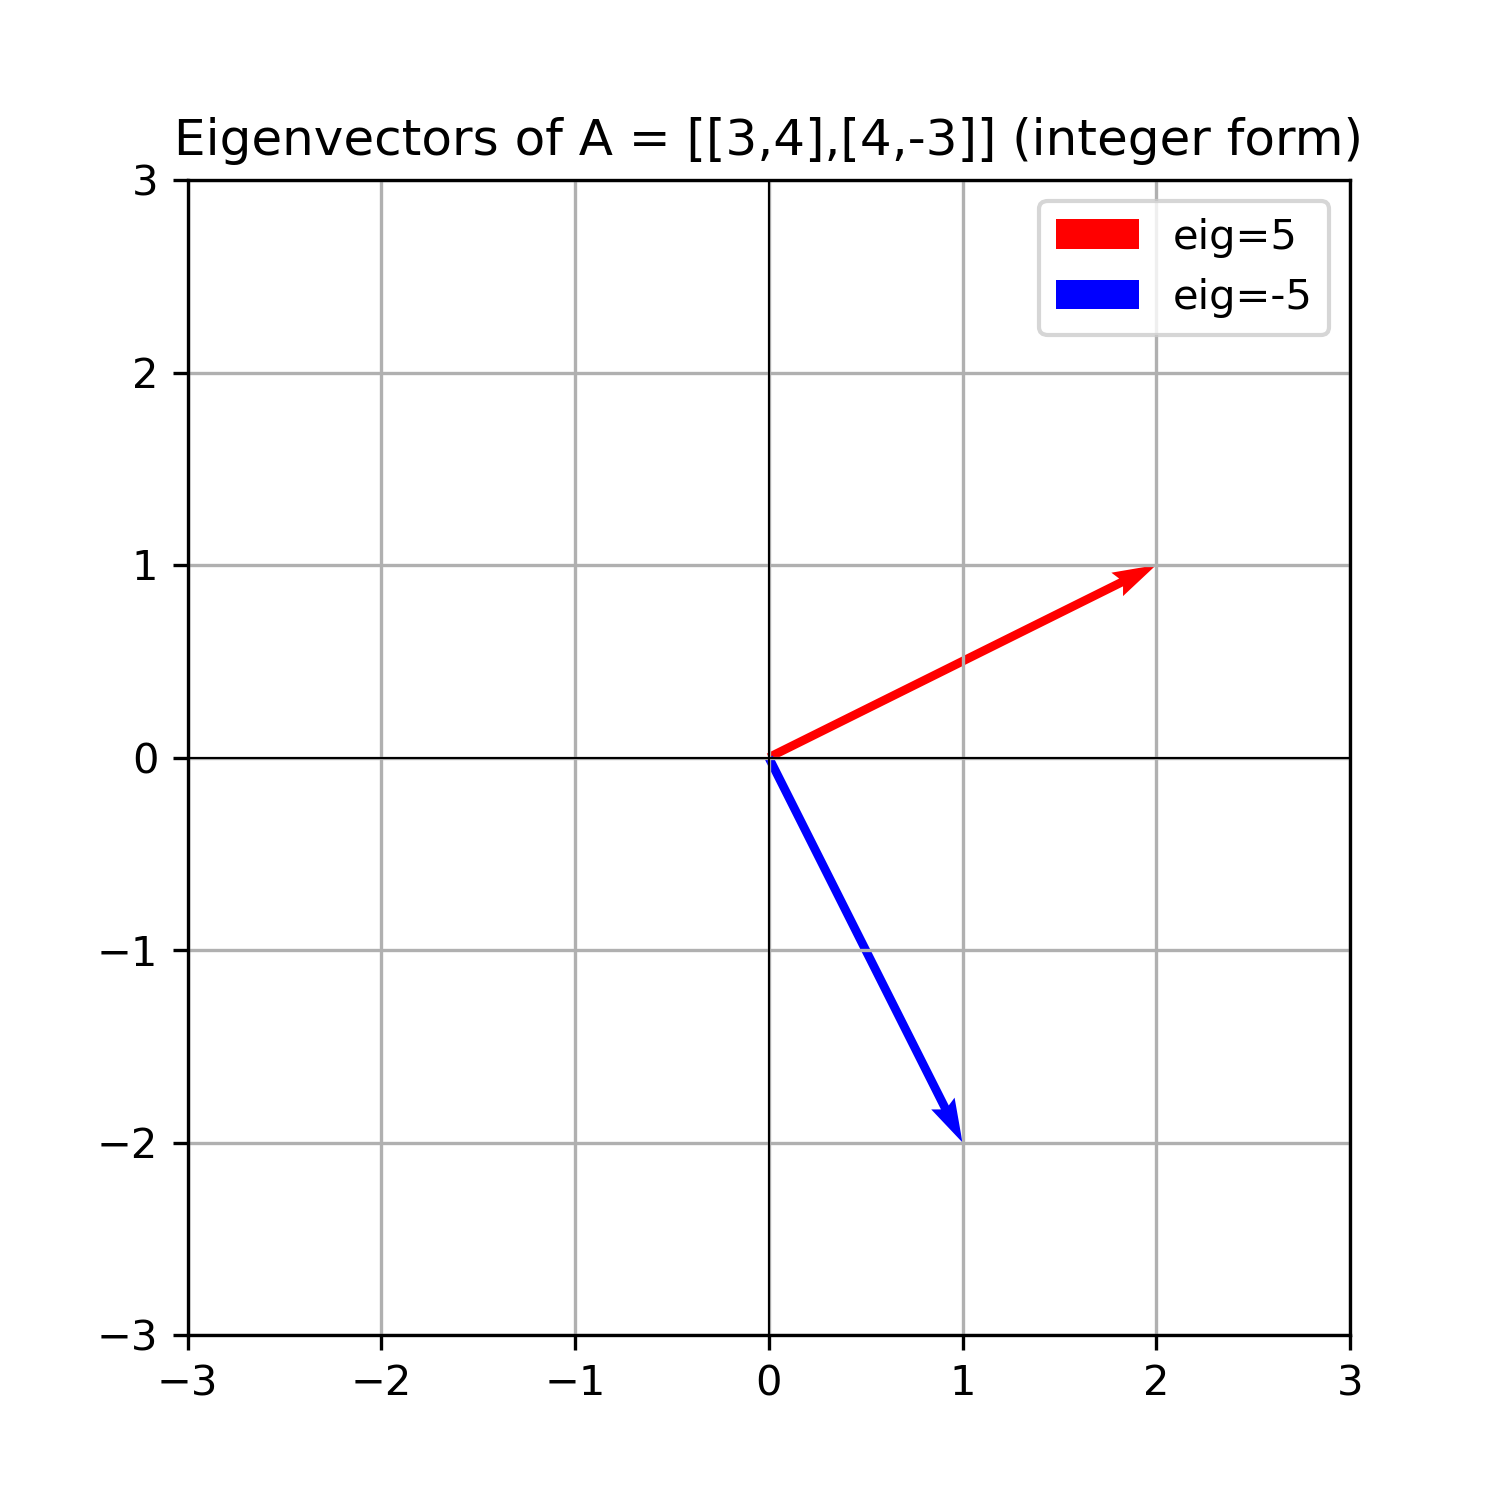
\includegraphics[width=0.6\columnwidth]{figs/eigenvectors_problem_adjusted.png}
   \caption{}
   \label{}
   \end{figure}
\end{frame}

\begin{frame}[fragile]
    \frametitle{Code - C}
    \begin{lstlisting}
#include <stdio.h>
#include <math.h>

// Compute eigenvalues of a 2x2 real matrix
// A = [a b; c d]
void eigenvalues(double a, double b, double c, double d, double *eig1, double *eig2) {
    double trace = a + d;
    double det = a * d - b * c;
    double disc = trace * trace - 4 * det;

    if (disc < 0) { // complex case not handled
        *eig1 = *eig2 = NAN;
        return;}
    *eig1 = (trace + sqrt(disc)) / 2.0;
    *eig2 = (trace - sqrt(disc)) / 2.0;
}




    \end{lstlisting}
    \end{frame}

    \begin{frame}[fragile]
    \frametitle{Code - C}
    \begin{lstlisting}
// Compute eigenvector for given eigenvalue
void eigenvector(double a, double b, double c, double d, double eig, double *v) {
    double m11 = a - eig;
    double m12 = b;
    double m21 = c;
    double m22 = d - eig;
    // Try first row equation: m11*x + m12*y = 0
    if (fabs(m11) > 1e-6 || fabs(m12) > 1e-6) {
        if (fabs(m12) > 1e-6) {
            v[0] = 1.0;
            v[1] = -m11 / m12;
        } else {
            v[0] = -m12 / m11;
            v[1] = 1.0;
        }
    }

    \end{lstlisting}
    \end{frame}

        \begin{frame}[fragile]
    \frametitle{Code - C}
    \begin{lstlisting}
    // Otherwise try second row
    else if (fabs(m21) > 1e-6 || fabs(m22) > 1e-6) {
        if (fabs(m22) > 1e-6) {
            v[0] = 1.0;
            v[1] = -m21 / m22;
        } else {
            v[0] = -m22 / m21;
            v[1] = 1.0;
        }
    } else {
        v[0] = v[1] = 0.0; // degenerate case
    }
}


    \end{lstlisting}
    \end{frame}

\begin{frame}[fragile]
    \frametitle{Code - Python(with shared C code)}
    The code to obtain the required plot is
    \begin{lstlisting}
import ctypes
import numpy as np
import matplotlib.pyplot as plt

# Load shared library
lib = ctypes.CDLL("./eigen.so")

# Define arg/return types
lib.eigenvalues.argtypes = [ctypes.c_double, ctypes.c_double,
                            ctypes.c_double, ctypes.c_double,
                            ctypes.POINTER(ctypes.c_double),
                            ctypes.POINTER(ctypes.c_double)]
lib.eigenvalues.restype = None

\end{lstlisting}
\end{frame}
\begin{frame}[fragile]
\frametitle{Code - Python(with shared C code)}
\begin{lstlisting}
lib.eigenvector.argtypes = [ctypes.c_double, ctypes.c_double,
                            ctypes.c_double, ctypes.c_double,
                            ctypes.c_double,
                            ctypes.POINTER(ctypes.c_double)]
lib.eigenvector.restype = None

# Example matrix A = [[3,4],[4,-3]]
a, b, c, d = 3.0, 4.0, 4.0, -3.0

eig1 = ctypes.c_double()
eig2 = ctypes.c_double()

# Get eigenvalues
lib.eigenvalues(a, b, c, d, ctypes.byref(eig1), ctypes.byref(eig2))
print("Eigenvalues:", eig1.value, eig2.value)



\end{lstlisting}
\end{frame}

\begin{frame}[fragile]
\frametitle{Code - Python(with shared C code)}
\begin{lstlisting}
vec1 = np.array([v1[0], v1[1]])
vec2 = np.array([v2[0], v2[1]])

print("Eigenvector for eig1:", vec1)
print("Eigenvector for eig2:", vec2)

# ---- Plot ----
plt.figure(figsize=(5,5))
plt.axhline(0, color="black", linewidth=0.5)
plt.axvline(0, color="black", linewidth=0.5)

plt.quiver(0, 0, vec1[0], vec1[1], angles='xy', scale_units='xy', scale=1,
           color="red", label=f"eig1={eig1.value:.2f}")
plt.quiver(0, 0, vec2[0], vec2[1], angles='xy', scale_units='xy', scale=1,
           color="blue", label=f"eig2={eig2.value:.2f}")


\end{lstlisting}
\end{frame}

\begin{frame}[fragile]
\frametitle{Code - Python(with shared C code)}
\begin{lstlisting}
plt.xlim(-3, 3)
plt.ylim(-3, 3)
plt.grid(True)
plt.legend()
plt.title("Eigenvectors of A = [[3,4],[4,-3]]")

# Save figure
plt.savefig("eigenvectors.png", dpi=300)

# Show figure
plt.show()

\end{lstlisting}
\end{frame}



\begin{frame}[fragile]
\frametitle{Code - Python only}
\begin{lstlisting}
import numpy as np
import matplotlib.pyplot as plt

# Define the matrix
A = np.array([[3, 4],
              [4, -3]], dtype=float)
# Compute eigenvalues and eigenvectors
eigvals, eigvecs = np.linalg.eig(A)
print("Matrix A:\n", A)
print("\nEigenvalues:", eigvals)
print("\nEigenvectors (normalized, from NumPy):\n", eigvecs)

# ---- Force integer eigenvectors ----
# For eig = +5, eigenvector ~ (2,1)
v1 = np.array([2, 1], dtype=float)
# For eig = -5, eigenvector ~ (1,-2)
v2 = np.array([1, -2], dtype=float)




\end{lstlisting}
\end{frame}

\begin{frame}[fragile]
\frametitle{Code - Python only}
\begin{lstlisting}
print("\nAdjusted Eigenvectors:")
print("Eigenvalue 5  :", v1)
print("Eigenvalue -5 :", v2)

# ---- Plot ----
plt.figure(figsize=(5,5))
plt.axhline(0, color="black", linewidth=0.5)
plt.axvline(0, color="black", linewidth=0.5)

plt.quiver(0, 0, v1[0], v1[1], angles='xy', scale_units='xy', scale=1,
           color="red", label="eig=5")
plt.quiver(0, 0, v2[0], v2[1], angles='xy', scale_units='xy', scale=1,
           color="blue", label="eig=-5")


\end{lstlisting}
\end{frame}

\begin{frame}[fragile]
\frametitle{Code - Python only}
\begin{lstlisting}
plt.xlim(-3, 3)
plt.ylim(-3, 3)
plt.grid(True)
plt.legend()
plt.title("Eigenvectors of A = [[3,4],[4,-3]] (integer form)")

# Save and show
plt.savefig("eigenvectors_problem_adjusted.png", dpi=300)
plt.show()




\end{lstlisting}
\end{frame}

\end{document}
